\subsection{Extending the Interface}
\label{sec:extending-interface}
With the |ArrowParallel| type class in place and implemented, we can now implement some further basic parallel interface functions. These are algorithmic skeletons that, however, mostly serve as a foundation to further, more specific algorithmic skeletons.

\subsubsection{Lazy |parEvalN|}
\begin{figure}[tb]
	\includegraphics[scale=0.7]{images/parEvalNLazy}
	\caption{Schematic depiction of |parEvalNLazy|.}
	\label{fig:parEvalNLazyImg}
\end{figure}
The function |parEvalN| is 100\% strict, which means that it fully evaluates all passed arrows. Sometimes this might not be feasible, as it will not work on infinite lists of functions like e.g. |map (arr . (+)) [1..]| or just because we need the arrows evaluated in chunks. |parEvalNLazy| (Figs.~\ref{fig:parEvalNLazyImg},~\ref{fig:parEvalNLazy}) fixes this. It works by first chunking the input from |[a]| to |[[a]]| with the given |ChunkSize| in |arr (chunksOf chunkSize)|. These chunks are then fed into a list |[arr [a] [b]]| of parallel arrows created by feeding chunks of the passed |ChunkSize| into the regular parEvalN by using |listApp|. The resulting |[[b]]| is lastly converted into |[b]| with |arr concat|.
\begin{figure}[t]
\begin{code}
parEvalNLazy :: (ArrowParallel arr a b conf, ArrowChoice arr, ArrowApply arr) =>
	conf -> ChunkSize -> [arr a b] -> (arr [a] [b])
parEvalNLazy conf chunkSize fs =
	arr (chunksOf chunkSize) >>>
    evalN fchunks >>>
    arr concat
    where
      fchunks = map (parEvalN conf) (chunksOf chunkSize fs)
\end{code} %$ %% formatting
\caption{Definition of |parEvalNLazy|.}
\label{fig:parEvalNLazy}
\end{figure}

\subsubsection{Heterogeneous tasks}
\begin{figure}[tb]
	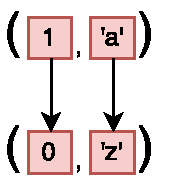
\includegraphics[scale=0.7]{images/parEval2}
	\caption{Schematic depiction of |parEval2|.}
	\label{fig:parEval2Img}
\end{figure}
We have only talked about the parallelisation of arrows of the same type until now. But sometimes we want to parallelize heterogeneous types as well. We can implement such a |parEval2| combinator (Figs.~\ref{fig:parEval2Img},~\ref{fig:parEval2}) which combines two arrows |arr a b| and |arr c d| into a new parallel arrow |arr (a, c) (b, d)| quite easily with the help of the |ArrowChoice| type class. The idea is to use the |+++| combinator which combines two arrows |arr a b| and |arr c d| and transforms them into |arr (Either a c) (Either b d)| to get a common arrow type that we can then feed into |parEvalN|.

%%% Local Variables:
%%% mode: latex
%%% TeX-master: "main"
%%% End:
